%%% LaTeX Template: Two column article
%%%
%%% Source: http://www.howtotex.com/
%%% Feel free to distribute this template, but please keep to referal to http://www.howtotex.com/ here.
%%% Date: February 2011

%%% Preamble
\documentclass[	DIV=calc,%
							paper=a4,%
							fontsize=12pt,%
							onecolumn]{scrartcl}	 					% KOMA-article class

\usepackage{lipsum}													% Package to create dummy text
\usepackage[english]{babel}										% English language/hyphenation
\usepackage[protrusion=true,expansion=true]{microtype}				% Better typography
\usepackage{amsmath,amsfonts,amsthm}					% Math packages
\usepackage[pdftex]{graphicx}									% Enable pdflatex
\usepackage[svgnames]{xcolor}									% Enabling colors by their 'svgnames'
\usepackage[hang, small,labelfont=bf,up,textfont=it,up]{caption}	% Custom captions under/above floats
\usepackage{epstopdf}												% Converts .eps to .pdf
\usepackage{subfig}													% Subfigures
\usepackage{booktabs}												% Nicer tables
\usepackage{fix-cm}													% Custom fontsizes
\usepackage[utf8]{inputenc}
\usepackage[top=2.5cm, bottom=2.5cm, left=2.5cm, right=2.5cm]{geometry}
\usepackage[ddmmyyyy]{datetime}
\addto\captionsenglish{%
	\renewcommand\tablename{Tabela}
	\renewcommand\figurename{Figura}
} 
 

 
%%% Custom sectioning (sectsty package)
\usepackage{sectsty}													% Custom sectioning (see below)
\allsectionsfont{%															% Change font of al section commands
	\usefont{OT1}{phv}{b}{n}%										% bch-b-n: CharterBT-Bold font
	}

\sectionfont{%																% Change font of \section command
	\usefont{OT1}{phv}{b}{n}%										% bch-b-n: CharterBT-Bold font
	}



%%% Headers and footers
\usepackage{fancyhdr}												% Needed to define custom headers/footers
	\pagestyle{fancy}														% Enabling the custom headers/footers
\usepackage{lastpage}	

% Header (empty)
\lhead{}
\chead{}
\rhead{}
% Footer (you may change this to your own needs)

%% ====================================
%% ====================================
%% mude o rodape  do projeto
%% ====================================
%% ====================================

\lfoot{\footnotesize \texttt{Etech Prestadora de Serviços - (43)999980797} \textbullet ~ Londrina / Pr.}


\cfoot{}
\rfoot{\footnotesize página \thepage\ de \pageref{LastPage}}	% "Page 1 of 2"
\renewcommand{\headrulewidth}{0.0pt}
\renewcommand{\footrulewidth}{0.4pt}



%%% Creating an initial of the very first character of the content
\usepackage{lettrine}
\newcommand{\initial}[1]{%
     \lettrine[lines=3,lhang=0.3,nindent=0em]{
     				\color{DarkGoldenrod}
     				{\textsf{#1}}}{}}



%%% Title, author and date metadata
\usepackage{titling}															% For custom titles

\newcommand{\HorRule}{\color{DarkGoldenrod}%			% Creating a horizontal rule
									  	\rule{\linewidth}{1pt}%
										}

\pretitle{\vspace{-12pt} \begin{flushleft} \HorRule 
				\fontsize{24}{24} \usefont{OT1}{phv}{b}{n} \color{DarkRed} \selectfont 
				}

%% ====================================
%% ====================================
%% mude o titulo  do projeto
%% ====================================
%% ====================================

\title{Projeto de cabeamento estruturado da empresa Etech ISP}					% Title of your article goes here

%% ====================================



\posttitle{\par\end{flushleft}\vskip 0.5em}

\preauthor{\begin{flushleft}
					\large \lineskip 0.5em \usefont{OT1}{phv}{b}{sl} \color{DarkRed}}
\author{André Giuliani RA 1909797 }  	% Author name goes here


\postauthor{\footnotesize \usefont{OT1}{phv}{m}{sl} \color{Black} 
					\\Universidade Tecnológica Federal do Paraná - Campus Cornélio Procópio
					\\Pós Graduação - Disciplina de Redes Estruturadas 								% Institution of author
					\par\end{flushleft}\HorRule}

\date{}																				% No date




%%% Begin document
\begin{document}
\maketitle
\thispagestyle{fancy} 	
\thispagestyle{empty}		% Enabling the custom headers/footers for the first page 
% The first character should be within \initial{}




%% ====================================
%% ====================================
%% mude o resumo  do projeto
%% ====================================
%% ====================================
\initial{E}\textbf
{	ste projeto visa atender a empresa de telecomunicações Etech ME no que se refere à estrutura interna para a rede lógica, esta rede compreenderá serviços de dados (Computadores e Servidores), voz (Telefones IP) e monitoramento de imagem (Cftv/IP). Trata-se de uma instalação nova sendo que no local ainda não há nenhuma infraestrutura pronta. Todos os pontos descritos serão atendidos cabos de rede Cat 6 que possuem capacidade de transmissão de até 10GBps, após a instalação todos os pontos serão aferidos pelo processo de certificação.}\\

\textbf
{	Conforme levantamento no local, junto aos sócios, a empresa está iniciando seus trabalhos como um pequeno provedor de internet via fibra no bairro Vila Casone em Londrina Pr., porém, apesar da estrutura inicial ser considerada pequena o projeto deverá contemplar futuras ampliações evitando custos desnecessários a posteriori; as futuras ampliações se limitarão ao patamar de duas vezes o tamanho da rede inicialmente implantada e deverão ser aplicadas a todos os passivos de rede pertinentes, tais como: Eletrocalhas, dutos, racks, quadros etc.}

%% ====================================
\begin{figure}
	\centering
	
\includegraphics{Etech}
\end{figure}

\vspace{3cm}
\centerline{\textit{\textbf{\today}}}

\clearpage
    \renewcommand*\listfigurename{Lista de figuras}
\listoffigures

\renewcommand*\listtablename{Lista de tabelas}
\listoftables




\clearpage
\renewcommand{\contentsname}{Sumário}
\tableofcontents
\clearpage

%% ====================================
%% ====================================
%% Inicio do texto
%% ====================================
%% ====================================
\section{Introdução}

%Explique nesta primeira seção qual seria o perfil do caso. Perfil do cliente, quantidade de colaboradores, quantidade de equipamentos de TI atualmente
Este projeto de cabeamento estruturado destina-se à empresa Etech ISP, trata-se de um provedor de pequena escala de serviços de comunicação multimídia e acesso á internet. Inicialmente a empresa conta com 5 colaboradores sendo 2 da área técnica, 2 administrativos e 1 comercial, cada colaborador utilizará em seu posto de trabalho um desktop e um telefone IP. Atualmente os recursos ativos de TI constam de:
Desktop Dell: 5 unidades;
Telefones IP Intelbrás: 6 unidades;
Servidor Dell: 1 unidade (No servidor estão virtualizados os serviços de Banco de dados, Aplicativo gerencial e Pabx IP); 
%Indique também nesta seção o escopo do projeto.
O propósito deste projeto é montar uma rede interna de alta capacidade e confiabilidade, com possibilidade de expansões futuras na proporção de 2 vezes o tamanho original.
%Apresente um overview do parque tecnológico do caso.


\subsection{Benefícios}
%Explique quais seriam os benefícios provenientes da execução deste projeto.
O sistema de cabeamento estruturado visa padronizar as instalações referentes a conectividade, trata-se de uma solução estratégica pois miniminiza custos de uma readequação física para mudanças de local no trabalho ou mesmo de novas instalações, segue os principais benefícios que a rede estruturada irá proporcionar:
\begin{itemize}
\item Suporte a diversos padrões de comunicação que utilizarão o mesmo meio físico, neste caso os sistemas de informática, telefonia e segurança irão utilizar o mesmo meio físico bem como o mesmo meio lógico utilizando o protocolo IP.
\item Facilidade na mudança de layout interno visto que as interfaces são padronizadas e os equipamentos portam suas respectivas configurações \item independente que qual local estejam conectados na rede.
\item Manutenção simples e rápida uma vez que todos os cabos e dispositivos são organizados e identificados em ambas extremidades.
\item Localização fácil de um cabo devido ao mesmo ser identificado por todo seu trajeto.
\item Documentação técnica que facilita a manutenção e novas implantações.
\end{itemize}
 
\section{Estado atual}

%Aprente o estado atual da rede. Caso não tenha rede, desconsiderar esta seção.
Atualmente a empresa é uma prestadora de serviços na área telemática e encontra-se em uma edícula que está atrás do novo prédio construído para abrigar a nova sede e os novos serviços, logo não será reaproveitado nenhum material, exceto os computadores e telefones IP utilizados atualmente.


%Caso tenha rede, deixe claro:
%os passivos de rede atuais:path panels, cabos, etc..;
%as principais reclamações dos usuários. Qual o principal motivo da reestruturação? Efetue uma pesquisa junto aos colaboradores para determinar quais problemas a rede apresenta.
%Observações. Analise a rede e verifique se há estruturas que não se enquadram nas normas ou que indicam suspeita de problemas.



\section{Usuários e Aplicativos}
Explique nesta seção os usuários atuais e o perfil de crescimento, se por exemplo, há estimativa na evolução da empresa no que tange a quantidade de usuários, pontos de redes, equipamentos.
 

\subsection{Usuários}
Crie uma relação da quantidade, perfil de usuários de seu projeto.

\subsection{Aplicativos}
Crie uma relação dos aplicativos e seus níveis críticos de uso.


\section{Estrutura predial existente}

Explique aqui a planta física dos prédios
Pode ser anexada, em escala ou não.

Deve conter uma descrição geral, indicando a possível distância entre os pontos de rede e restrições de instalação.

\section{Planta Lógica - Elementos estruturados}

\subsection{Estado atual}
Deve ter a planta atual, se for o caso

\subsection{Topologia}
Proposta futura, proposta após implantação.
Deve conter o diagrama da rede. Atente-se a redundância  e ligações truncadas.
Deve explicar todos termos e componentes utilizados nestas plantas. Por exemplo: entrance facility, work area, horizontal cabling, etc..

Todos os elementos das figuras devem ser explicados. 
Crie esboço da configuração dos racks e brackets. Explique cada um dos componentes. Você pode criar uma tabela contendo figuras dentro, ou criar uma tabela e incluí-la como imagem. Por exemplo, verifique a tabela \ref{tab1}.

\begin{table}[h!]
\centering
\caption{Exemplo de tabela explicativa}
\label{tab1}
\begin{tabular}{|l|l|l|}
\hline
\multicolumn{3}{|l|}{Figura na Tabela} \\ \hline
1        & Rack          & \includegraphics[scale=0.2]{fig1}        \\ \hline
2        & Rack 2        & \includegraphics[scale=0.2]{fig1}        \\ \hline
\end{tabular}
\end{table}

\subsection{Encaminhamento}
Eletrodutos, calhas, e qualquer material em que os cabos serão alojados/alocados.

\subsection{Memorial descritivo}

Relacione todos os equipamentos passivos que serão utilizados, tipo, fabricante, quantidade.

\subsection{Identificação dos cabos}

\section{Implantação}
Estabeleça um cronograma de implantação:
Remoção de equipamentos existentes (destino para descarte), instalação dos condutores, instalação dos cabos, 
identificação dos cabos, montagem dos racks, certificação, etc... Crie atividades e estabeleça o tempo de execução. Se for um projeto real, indique também quais os responsáveis pela execução do projeto e de cada uma das etapas.

Defina marcas (e padrões) e fornecedores se for o caso. Atenção a contratados e subcontratados para a realização das atividades. Estabeleça a responsabilidade de execução da atividade e também da validação dela.

Utilize algum software para gerear o cronograma. Excel,etc. O fundamental é dividir em etapas, descrever e estimar o tempo de cada uma delas.

Segue uma relação de ferramentas:
http://asana.com/, 
https://trello.com/, 
http://www.ganttproject.biz/, 
http://www.orangescrum.org/. 

\section{Plano de certificação}
Quais seriam as etapas para a certificação? 
Quais os locais e horários para execução da certificação na rede? Toda rede será certificada?
Como os testes seriam executados?
Quais relatórios de certificação serão (ou deveriam ser) entregues? 

\section{Plano de manutenção}

Revisões periódicas na rede, emissão de certificados para novos pontos.

\subsection{Plano de expansão}
Existe um plano de expansão? Quantos novos pontos poderão ser acrecidos na rede, antes de migração de equipamentos na camada 2? Se houver expansão, quais equipamentos deverão ser direcionados para as estremidades da rede? 


\section{Orçamento}
Crie uma relação de orçamentos baseado na seções anteriores.

\section{Referências bibliográficas}
Utilize o mendley, o jabref ou diretamente o bibtex para gerenciar suas referências biliográficas. As referências são criadas automaticamente de acordo com o uso no texto.

Exemplo: Redes de computadores, segundo \cite{t2013} é considerada..... Já \cite{kurose2010} apresenta uma versão...

Analisando os pressupostos de \cite{ref3} e \cite{ref4} concluimos que....


\renewcommand\refname{} %%Referências bibliográficas}  
\bibliographystyle{ieeetr}
\bibliography{referencias}  

%% ***********************************************************************
%% === remover daqui =====================================================
%% ***********************************************************************

\section{Elementos textuais - Alguns exemplos}

Esta seção apresenta exemplos de elementos textuais. \textbf{Remova-a da versão final do texto}.


\subsection{Colocar elementos em itens}

Texto antes da lista

\begin{itemize}
	\item First item in a list 
	\item Second item in a list 
	\item Third item in a list
\end{itemize}

\subsubsection{Uma sub seçao de terceiro nivel}

Exemplo de uma subseção

\subsection{Tabelas}

Utilize o site http://www.tablesgenerator.com/ para elaborar as tabelas de seu trabalho.
Para adicionar uma tabela utilize: a tag input, passando o arquivo da tabela como parametro

\begin{table}[h!] % coloque h! para forcar a posicao
\centering
\caption{Modifique a legenda e crie um label}
\label{tab2} %com este label vc faz referencia no texto
\begin{tabular}{|l|l|l|l|l|}
\hline
\multicolumn{1}{|c|}{\textbf{Este é um exemplo de tabela}} & \multicolumn{2}{c|}{\textbf{C1}} & \multicolumn{2}{c|}{\textbf{C2}} \\ \hline
Você pode criar a tabela no excel                          & 1              & 2               & 3               & 4              \\ \hline
Exportar para CSV                                          & 5              & 6               & 7               & 8              \\ \hline
E importar no Table Generator                              & 9              & 10              &                 &                \\ \hline
\multicolumn{5}{|c|}{\textit{Gere o tex, e adicione em seu arquivo}}                                                             \\ \hline
\end{tabular}
\end{table}

Dentro do arquivo você deve definir o label e pode utilizá-lo para referenciar. Exemplo:
Na tab \ref{tab2} temos a relação de ....


Você também pode modificar a tabela manualmente, incluindo, por exemplo h! dentro de sua definição. Veja no exemplo tab2.tex

\subsection{Figuras}

As figuras podem ser no formato PDF, JPG, PNG. Você pode referenciá-las da mesma maneira que tabelas. Exemplo: A figura \ref{fig1} apresenta.....

Não se preocupe o local em que a figura será renderizada em seu texto. Preocupe-se em criar referência para ela, ou seja, toda figura e tabela deve conter pelo menos uma referência no texto.

\begin{figure}
\centering
\includegraphics[width=\textwidth]{fig1}
\caption{Exemplo de figura com escala horizontal}
\label{fig1}
\end{figure}


\begin{figure}
	\centering
	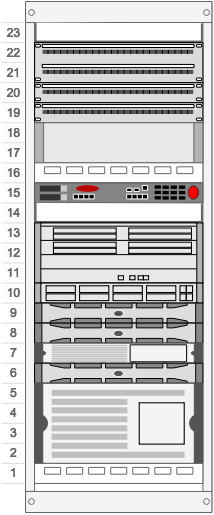
\includegraphics[]{fig2}
	\caption{Exemplo de figura sem escala}
	\label{fig2}
\end{figure}

Você pode rotacionar figuras também. Para isso utilize o parâmetro angle=-90. Repare que a escala da figura foi modificada pelo parametro height. Você também pode utilizar scale

\begin{figure}
	\centering
	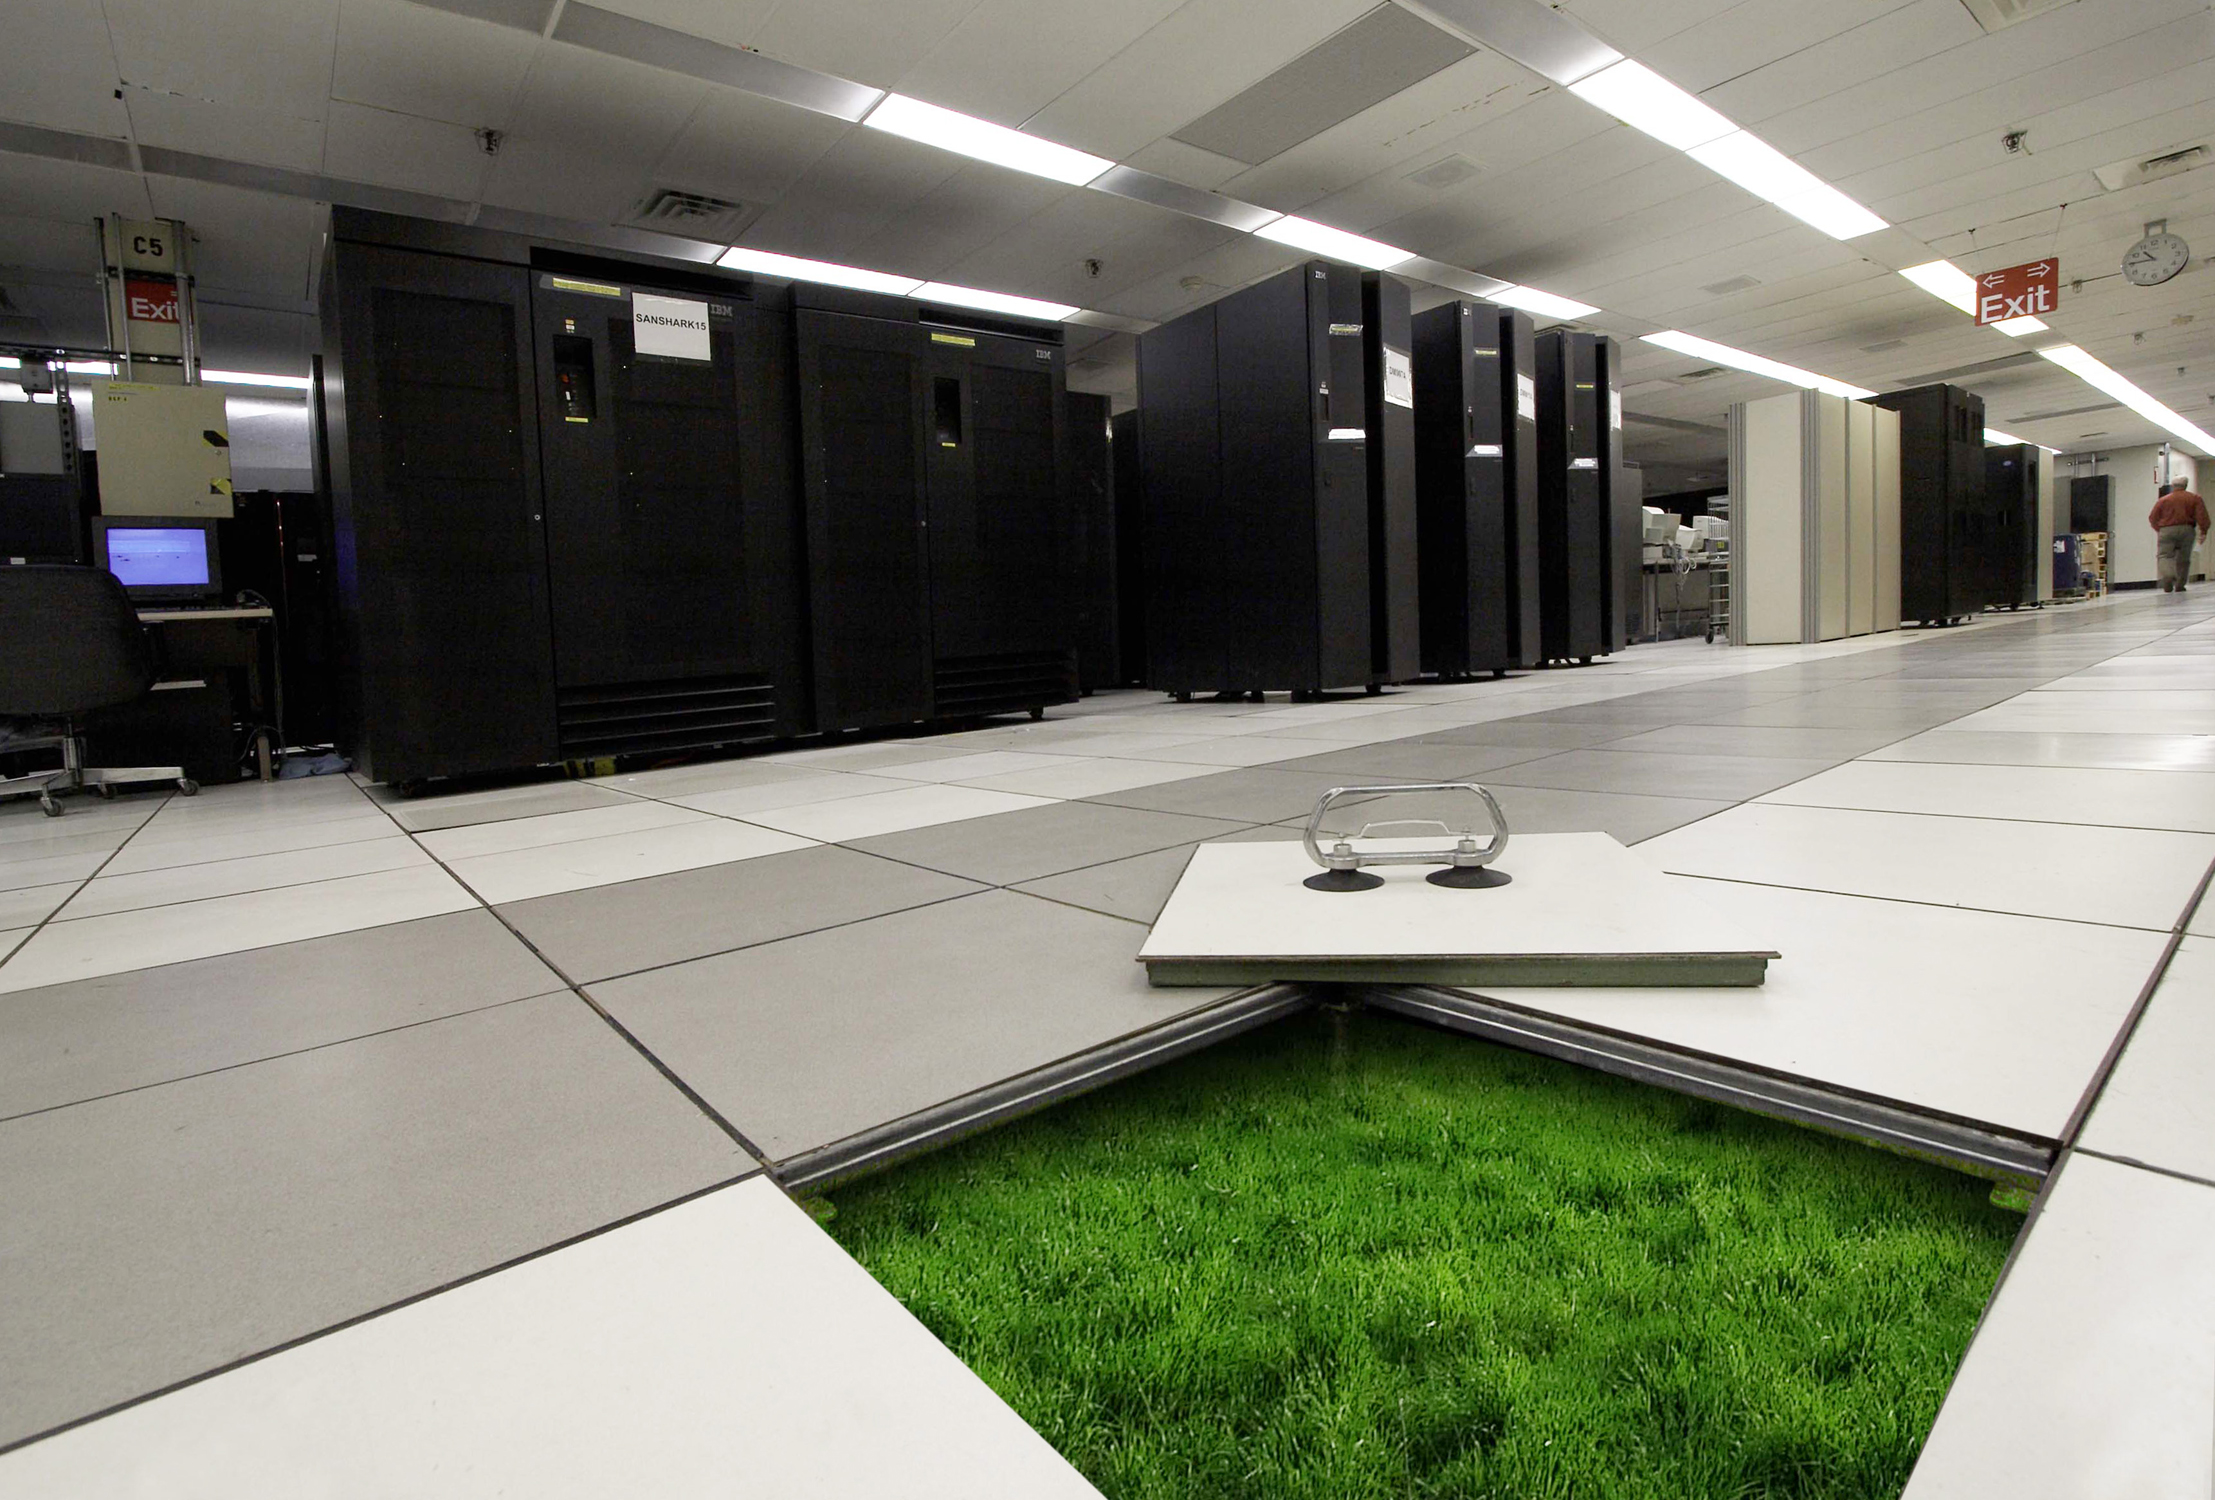
\includegraphics[height=\textwidth,angle=-90]{fig3}
	\caption{Exemplo de figura rotacionada}
	\label{fig3}
\end{figure}


%% ***********************************************************************
%% === ate aqui    =====  ================================================
%% ***********************************************************************
\end{document}